\chapter{Motion planning}
\label{chap:motion_planning}

\section{Existing local planner algorithms}
\label{chap:existing_local_planner_algorithms}
After building a map of the static and dynamic objects surrounding the vehicle, the next step is motion planning, which consists of two sub-tasks - global trajectory planning and local obstacle avoidance. As a result of global planning, a trajectory is created that - without taking the moving obstacles into consideration - leads the car to the target configuration, without making it collide with any static objects in the way. Local obstacle avoidance takes this trajectory as its input, and updates the car's actuators (acceleration and steering) to follow this trajectory, while also preventing collisions with dynamic objects.

As a part of my diploma project, I implemented the latter, a local obstacle avoidance algorithm, that relies on the previously created static and dynamic maps, and gets its input trajectory from a global planner node\footnote{Implementing a global motion planner was not part of my diploma project, but is considered a necessary condition for the local planner to work properly.}. According to \cite{DynamicMotionPlanningSurvey}, there exists a wide range of local planner algorithms, and they can easily be grouped by their complexity:

\begin{itemize}
  \item Velocity-based methods, most of the times combined with the dynamic window approach
  \item Predictive and probability-based methods
  \item Complex methods based on visual detection and AI
  \item Other methods
\end{itemize}

Out of these methods, velocity-based algorithms are by far the most popular, due to their being relatively easy to comprehend and implement and because of their low hardware requirements. As the mapping node and the local planner that I designed need to run on a processor with limited resources, I also chose a velocity-based obstacle avoidance method, using velocity obstacles, with dynamic windowing.

After reading about several motion planning algorithms, I found two different approaches that I thought was worth looking into more deeply.

One was the collision cone approach explained in \cite{CollisionCone}. This algorithm creates a cone that is designed in a way that it encloses the vehicle and also the obstacle it needs to avoid (see Figure \ref{collision_cones}). The cone defines how probable a collision is to happen using a given speed relative to the other object.

\begin{figure}[!ht]
    \centering
    \subfloat[Between point and circle]
    {
        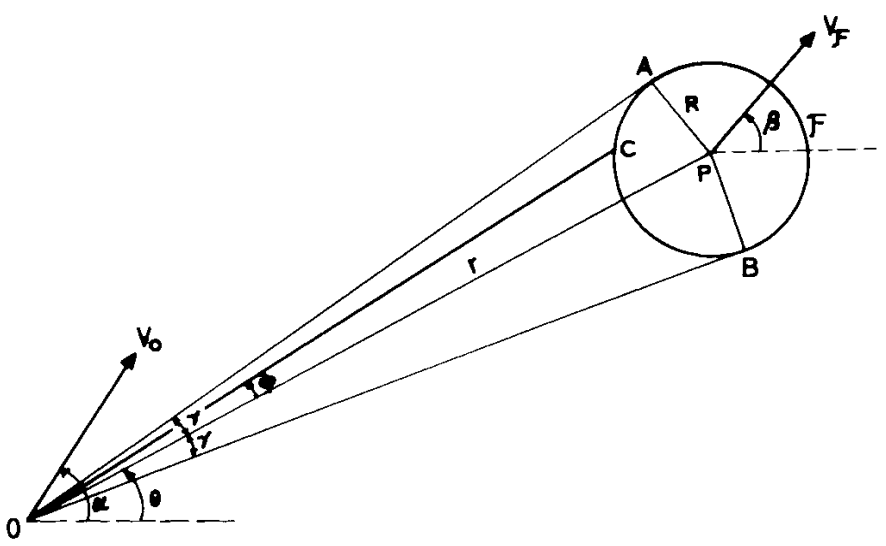
\includegraphics[height=48mm]{figures/raw/collision_cone_point_circle.png}
        \label{collision_cone_point_circle}
    }
    \subfloat[Between point and irregular geometry]
    {
        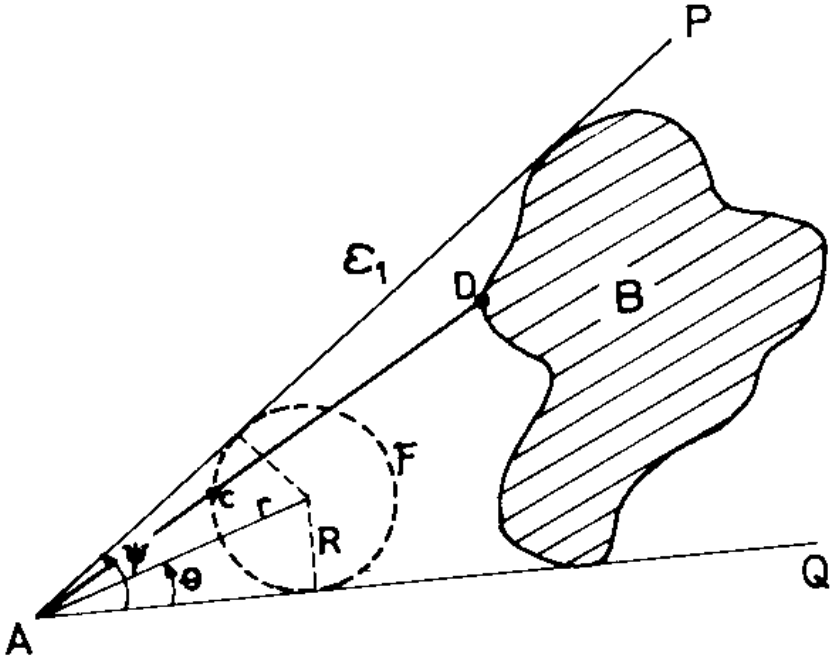
\includegraphics[height=48mm]{figures/raw/collision_cone_point_irregular_geometry.png}
        \label{collision_cone_point_irregular_geometry}
    }
    \caption{Collision cones}
    \label{collision_cones}
\end{figure}

The other method was to use velocity obstacles (described in \cite{VelocityForbiddenMap} and in \cite{VelocityObstacles}). These methods are based on the following statement: \textit{Assuming a given a given vehicle configuration (position, orientation, speed and wheel angle), the time until collision with a given static or dynamic object in the map can be calculated.} Therefore, velocity obstacle-based methods calculate this collision time for all surrounding objects and for all vehicle velocities. thus creating a velocity obstacle map, or forbidden velocity map (also referred to as dynamic velocity space in \cite{DynamicMotionPlanningSurvey}) that defines how safe given velocities are. Another implementation is explained in \cite{ReactivePathPlanning}, where the above mentioned two approaches are mixed while creating a virtual plane that enables the car to navigate in a dynamic environment.

\section{Method}
The planner algorithm I implemented uses velocity obstacles to determine which configurations of the car are safe.  Using the dynamic window approach is advised in this step, as it filters out non-reachable velocities before collision-time calculations, thus decreasing the execution time of the algorithm.

Given this velocity obstacle map, the algorithm has a basic knowledge of the reachable velocities and their level of safety. These safety levels provide a good starting point for further calculations, trajectory and collision estimations. My algorithm converts the forbidden velocity map's collision times to safety factors, but also takes the destination point's position and the target speed into consideration when selecting the next actuator outputs. The next graph shows all the sub-tasks of the local trajectory planner algorithm.

\tikzset{
  base_node/.style     = {rectangle, rounded corners, draw=black,
                          minimum width=4.5cm, minimum height=1cm,
                          text centered, font=\sffamily},
  inout_node/.style    = {base_node, fill=blue!30, minimum width=3.0cm},
  update_node/.style   = {base_node, fill=orange!15},
  dynamic_node/.style  = {base_node, fill=red!30},
  static_node/.style   = {base_node, fill=yellow!30},
  velo_obs_node/.style = {base_node, fill=green!30},
  decoration={brace},
  tuborg/.style={decorate},
  tubnode_left/.style={midway, left=2pt},
  tubnode_right/.style={midway, right=2pt}
}

\begin{center}
    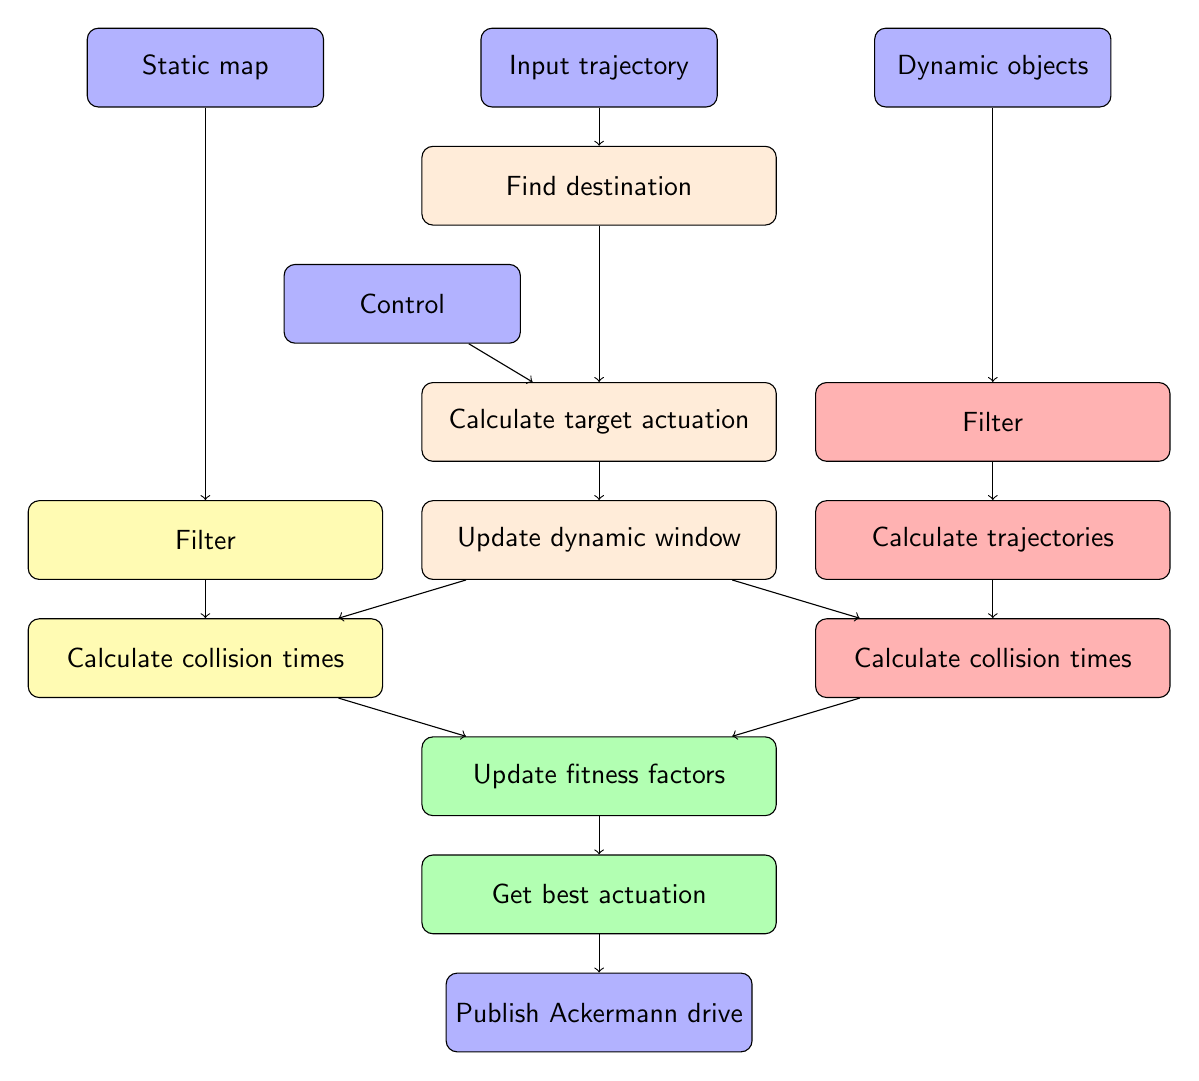
\begin{tikzpicture}[
            node distance=1.5cm,
            every node/.style={fill=white, font=\sffamily}, align=center]
        % Input nodes
        \node (static_map)      [inout_node]                                            {Static map};
        \node (trajectory)      [inout_node, xshift=5.0cm]                              {Input trajectory};
        \node (control)         [inout_node, xshift=2.5cm, yshift=-3.0cm]               {Control};
        \node (dynamic_objects) [inout_node, xshift=10.0cm]                             {Dynamic objects};
        % Update nodes
        \node (find_dest)       [update_node, below of=trajectory]                      {Find destination};
        \node (calc_target_act) [update_node, below of=find_dest, yshift=-1.5cm]        {Calculate target actuation};
        \node (update_window)   [update_node, below of=calc_target_act]                 {Update dynamic window};
        % Static nodes
        \node (static_filter)   [static_node, below of=static_map, yshift=-4.5cm]       {Filter};
        \node (static_calc_col) [static_node, below of=static_filter]                   {Calculate collision times};
        % Dynamic nodes
        \node (dynamic_filter)  [dynamic_node, below of=dynamic_objects, yshift=-3.0cm] {Filter};
        \node (dynamic_traj)    [dynamic_node, below of=dynamic_filter]                 {Calculate trajectories};
        \node (dyn_calc_col)    [dynamic_node, below of=dynamic_traj]                   {Calculate collision times};
        % Velocity obstacle nodes
        \node (fitness_factors) [velo_obs_node, below of=update_window, yshift=-1.5cm]  {Update fitness factors};
        \node (get_best_act)    [velo_obs_node, below of=fitness_factors]               {Get best actuation};
        \node (acker_drive)     [inout_node, below of=get_best_act]                     {Publish Ackermann drive};
        % Static connections
        \draw[->]      (static_map) -- (static_filter);
        \draw[->]   (static_filter) -- (static_calc_col);
        % Update connections
        \draw[->]      (trajectory) -- (find_dest);
        \draw[->]         (control) -- (calc_target_act);
        \draw[->]       (find_dest) -- (calc_target_act);
        \draw[->] (calc_target_act) -- (update_window);
        \draw[->]   (update_window) -- (static_calc_col);
        \draw[->]   (update_window) -- (dyn_calc_col);
        % Dynamic connections
        \draw[->] (dynamic_objects) -- (dynamic_filter);
        \draw[->]  (dynamic_filter) -- (dynamic_traj);
        \draw[->]    (dynamic_traj) -- (dyn_calc_col);
        % Velocity obstacle connections
        \draw[->] (static_calc_col) -- (fitness_factors);
        \draw[->]    (dyn_calc_col) -- (fitness_factors);
        \draw[->] (fitness_factors) -- (get_best_act);
        \draw[->]    (get_best_act) -- (acker_drive);
    \end{tikzpicture}
    \captionof{figure}{Motion planning method}
    \label{motion_planning_method}
\end{center}

The diagram consists of 4 sub-graphs - these are also marked on the diagram with different colors. The orange sub-graph describes the environment-independent sub-tasks of the algorithm - finding the next destination point, updating the target actuation and the dynamic window. The yellow one is about the method of reducing the size of the static map by filtering out those points that are not needed for the trajectory planning. The red side sub-graph shows that for dynamic objects, trajectory calculation is also necessary besides filtering. And the last one (populating the bottom area of the graph, marked with green colour) contains the main planning logic. The sections under \ref{chap:motion_planning} explain these sub-graphs in detail.

\begin{minipage}{\textwidth}
\section{Input parameters}
\label{chap:motion_planner_input_parameters}
The following input parameters can manipulate the motion planning node:

\begin{itemize}
\item\textbf{CAR\_FRONT\_REAR\_WHEEL\_AXIS\_DIST} [meter] The distance between the front and rear wheels axles of the car.
\item\textbf{CAR\_LENGTH} [meter] The length of the car.
\item\textbf{CAR\_WIDTH} [meter] The width of the car.
\item\textbf{COLLISION\_CHECK\_TIME\_STEP} [millisecond] The resolution of the iterative collision check.
\item\textbf{DYNAMIC\_WINDOW\_ANGLE\_RESOLUTION} [radian] The wheel angle resolution of the dynamic window.
\item\textbf{DYNAMIC\_WINDOW\_SPEED\_RESOLUTION} [meter/sec] The speed resolution of the dynamic window.
\item\textbf{MAX\_ACCELERATION} [meter/sec2] The maximum permitted acceleration.
\item\textbf{MAX\_DYNAMIC\_OBSTACLE\_DISTANCE} [meter] The radius of the dynamic obstacle filter.
\item\textbf{MAX\_SPEED\_BWD} [meter/sec] The maximum permitted backward speed.
\item\textbf{MAX\_SPEED\_FWD} [meter/sec] The maximum permitted forward speed.
\item\textbf{MAX\_STATIC\_OBSTACLE\_DISTANCE} [meter] The radius of the static obstacle filter.
\item\textbf{MAX\_WHEEL\_ANGLE} [radian] The maximum permitted wheel angle. 
\item\textbf{MAX\_WHEEL\_ANGULAR\_VELOCITY} [radian/sec2] The maximum permitted angular velocity of the steered wheels.
\item\textbf{MIN\_KEPT\_DISTANCE} [meter] The minimum distance to keep from objects
\item\textbf{W\_DIRECTION\_FACTOR} [dimensionless] The weight of the direction factor when finding the best possible actuation.
\item\textbf{W\_SAFETY\_FACTOR} [dimensionless] The weight of the safety factor when finding the best possible actuation.
\item\textbf{W\_SPEED\_FACTOR} [dimensionless] The weight of the speed factor when finding the best possible actuation.
\end{itemize}
\end{minipage}

\section{Target actuation and dynamic window}
\label{chap:target_actuation_and_dynamic_window}
In every loop (at each new incoming map data), the target actuation and the dynamic window are updated. The target actuation describes the desired speed and steering wheel angle for the next step, therefore the desired linear and angular speed vectors. The dynamic window is independent from the target actuation, but depends on the current actuation. It contains a set of speeds and wheel angles that are reachable by the car within the next step. The width and height of the window (the maximum speed and wheel angle change in one step) are defined by the mechanical characteristics of the car. So basically, the aim of this sub-task is to provide the algorithm a target actuation, and a set of reachable actuations.

When I implemented the target actuation update mechanism, that leads the car according to the input trajectory, I had several options to choose from. The first option was to split the trajectory into line-segments, and implement and tune a steering angle controller (e.g. a PD controller) to follow this line. I dropped this idea to prevent the re-tuning that would have been needed for each target vehicles (simulation, real-life test vehicles). Another option was the 'invisible string' the 'dog bone' method, where a target destination point is always in front of the car, and the car is always trying to reach this point, as if the point was pulling it by a string. The target actuation's wheel angle defines a trajectory curve, that goes through the destination point. If the destination point is always on the trajectory, and in front of car (within the right distance range), the car is going to follow the trajectory. I chose the latter (the 'invisible string') method.

\subsection{Finding the next destination point}
This method requires a destination point in each iteration. This point is preferably on the trajectory, in front of the car, 'pulling' the car to the right direction. The destination point search starts with finding the point in the trajectory nearest to the car's current position. The destination point needs to be in front of the car, but its distance from the car (which is nearly equal to its distance from the previously found nearest point) is not trivial (see Figure \ref{dest_point_update}).

\begin{figure}[!ht]
    \centering
    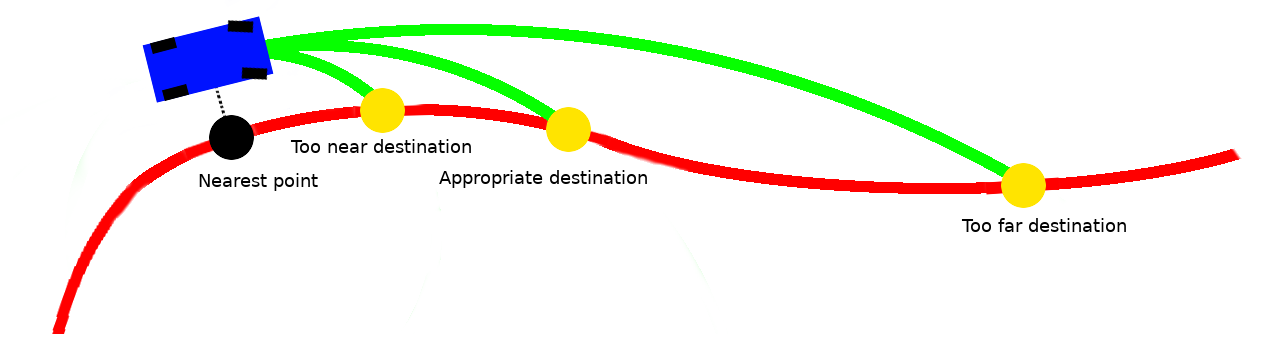
\includegraphics[height=40mm]{figures/raw/dest_point_update.png}
    \caption{Updating the destination point}
    \label{dest_point_update}
\end{figure}

Choosing a too near destination will result in the car starting to oscillate around the target trajectory with an increasing amplitude, until a point where the angular difference between the car and the trajectory will be too large for the car to find the path again. This situation is displayed in Figure \ref{traj_oscillation}.

\begin{figure}[!ht]
    \centering
    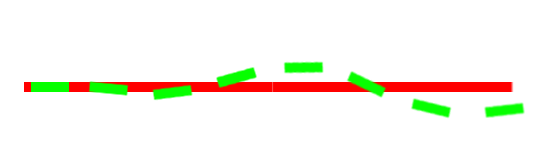
\includegraphics[width=65mm]{figures/raw/traj_oscillation.png}
    \caption{Oscillation around the target trajectory}
    \label{traj_oscillation}
\end{figure}

However, the destination point must not be chosen too far, either, because it straightens the curves of the trajectory, rounds its sharp peaks, and adds an offset to the long circular sections. Figure \ref{traj_rounding} demonstrates these effects. The effect shown on the left side might even be advantageous, but the right-hand side effect is certainly not.

\begin{figure}[!ht]
    \centering
    \subfloat[Rounding sharp peaks]
    {
        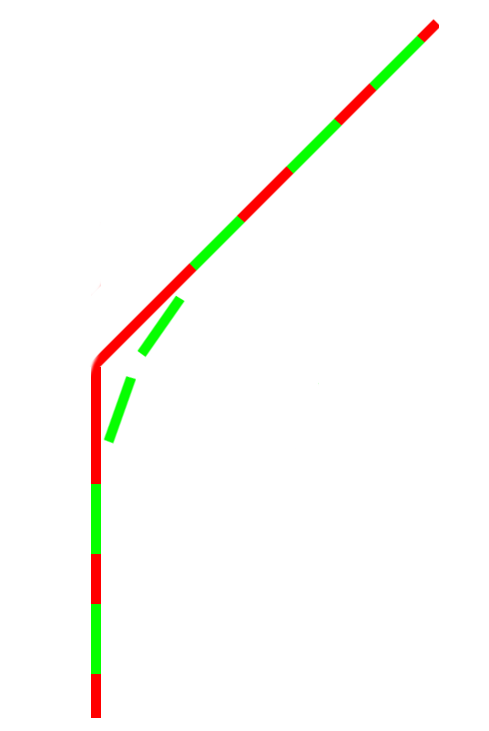
\includegraphics[height=72mm]{figures/raw/traj_round_sharp_peak.png}
        \label{traj_round_sharp_peak}
    }
    \subfloat[Rounding curves]
    {
        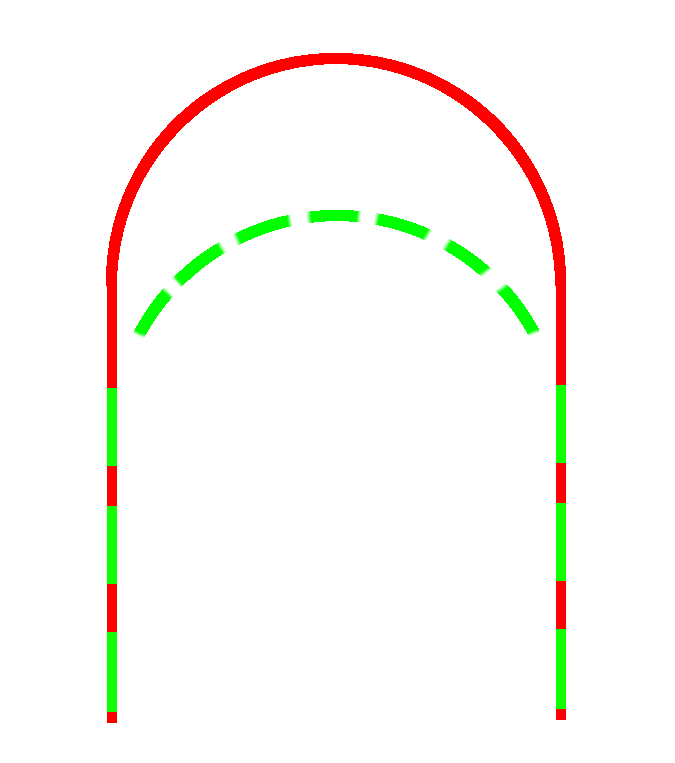
\includegraphics[height=72mm]{figures/raw/traj_round_curve.png}
        \label{traj_round_curve}
    }
    \caption{Trajectory rounding}
    \label{traj_rounding}
\end{figure}

After empirical testing, the optimal distance of the destination point and the nearest trajectory point (marked with yellow and black dots in Figure \ref{dest_point_update}) proved to be around 4 times the distance between the car's front and rear axles (see CAR\_FRONT\_REAR\_WHEEL\_AXIS\_DIST in Section \ref{chap:motion_planner_input_parameters}). Note, that this value largely depends on the dynamic window's maximum angular velocity limit and the car's mechanical characteristics (e.g. using a faster steering servo or a 4-wheel steering car would reduce the optimal distance).
In order to follow the straight segments of the target path before curves, I implemented the length of the invisible string (the distance in front of the nearest trajectory point) to change dynamically, according to the car's current distance from the trajectory. This tweak suppressed the rounding effect mentioned above, but not entirely. This is now considered a limitation of the algorithm's efficiency.

\subsection{Calculating the target actuation}
After the destination point has been selected, the next step is to calculate the target actuation - the speed and steering angle pair that would lead the car to the destination point. First, the target wheel angle is calculated using simple geographic considerations (see Figure \ref{calc_steering_angle}). The target speed calculation is based on two factors. The first is the target speed limit, which we expect the car to keep, given no extraordinary circumstances. This should be set to a safe speed that the car can keep up during its travel (see MAX\_SPEED\_FWD and MAX\_SPEED\_BWD in Section \ref{chap:motion_planner_input_parameters}). The actual target speed will never exceed this limit. But the target steering angle may require this target speed to be lower, because the car can manage to reach higher speeds safely when going straight, but not in a sharp bend.

\begin{figure}[!ht]
    \centering
    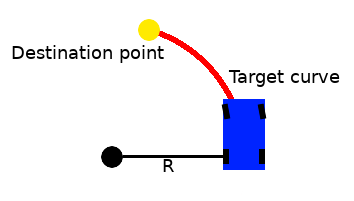
\includegraphics[height=48mm]{figures/raw/calc_steering_angle.png}
    \caption{Calculating the target steering angle}
    \label{calc_steering_angle}
\end{figure}

\subsection{External target actuation}
For easier testing, the node also supports external target actuations, meaning that the target actuation is not calculated from a trajectory, but is directly provided by another node. The external actuation can be set on topic \textit{/vrcar/filtered\_control\_orig}, which is a topic of \href{http://docs.ros.org/jade/api/ackermann_msgs/html/msg/AckermannDrive.html}{\textit{ackermann\_msgs/AckermannDrive}} messages, that have the following layout:

\begin{minipage}{\textwidth}
\begin{lstlisting}[language=IDL]
float32 steering_angle
float32 steering_angle_velocity
float32 speed
float32 acceleration
float32 jerk
\end{lstlisting}
\end{minipage}

Among other fields (which are currently not used by the project) it has a \textit{speed} and a \textit{steering\_angle} field - given in m/s and radians. These two fields are used as the target speed and wheel angle.

The program chooses between the target actuation modes dynamically, and the external target actuation has greater priority. So when messages are arriving on the external target actuation topic, they are the ones the algorithm uses, but when these messages cease to arrive, the node automatically switches to trajectory follow mode and calculates the next target actuation according to the given path.

\subsection{Updating the dynamic window}
In every iteration, the dynamic window must also be updated, which is independent from the target actuation, but depends on the current actuation, which is obtained by reading the odometry message published another node in the car. I have already described the structure of the \href{http://docs.ros.org/melodic/api/nav_msgs/html/msg/Odometry.html}{\textit{\textit{nav\_msgs/Odometry}}} message earlier in Section \ref{chap:absolute_points}.

The 'width' and 'height' of the window (which is defined by the maximum speed and wheel angle change in one iteration) mostly depends on the car's physical, mechanical and other characteristics (motor-wheel dead-time, maximum motor torque, speed controller's parameters, maximum angular velocity of the steering servo), but the environment's characteristics (air resistance, friction) also influence them. The maximum speed and wheel angle change are settable parameters (see MAX\_ACCELERATION and MAX\_WHEEL\_ANGULAR\_VELOCITY in Section \ref{chap:motion_planner_input_parameters}). The dynamic window is represented in Figure \ref{dynamic_window}. The red arrow shows the current actuation (speed and wheel angle pair). The dynamic window itself appears on the image as the grey area under the arrow heads. Every actuation within the dynamic window's area is reachable within the next step. When the current actuation is not near a hard limit, it is the center of the dynamic window.

\begin{figure}[!ht]
    \centering
    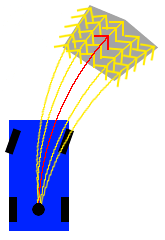
\includegraphics[height=60mm]{figures/raw/dynamic_window.png}
    \caption{The dynamic window}
    \label{dynamic_window}
\end{figure}

However, the size of the dynamic window may reduce when its size is limited by the hard limits of speed and wheel angle. A perfect example for this situation is when the steering angle is at its maximum at either left or right direction (see MAX\_WHEEL\_ANGLE in Section \ref{chap:motion_planner_input_parameters}), in which case changing the angle further to this direction is impossible. This results in the dynamic window getting halved - as only its original right or left side is reachable, depending on the current steering direction. It is trivial that in these cases such as the previous example, the current actuation is no longer in the center of the dynamic window.
Another important characteristics of the dynamic window is its resolution - both speed and angular velocity, which are settable parameters (see DYNAMIC\_WINDOW\_SPEED\_RESOLUTION and DYNAMIC\_WINDOW\_ANGLE\_RESOLUTION in Section \ref{chap:motion_planner_input_parameters}). Increasing the resolution leads to smoother control, but also increases the node's resource need and runtime.

The motion planning node also publishes the dynamic window's possible actuations in a \href{http://docs.ros.org/melodic/api/visualization_msgs/html/msg/MarkerArray.html}{\textit{visualization\_msgs::MarkerArray}} on topic \textit{available\_velocities}, so that they can be viewed on-the-fly in rviz.

\begin{figure}[!ht]
    \centering
    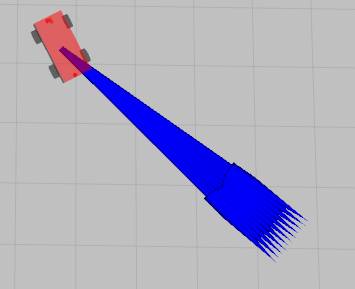
\includegraphics[height=60mm]{figures/raw/rviz_available_velocities.png}
    \caption{Available velocities in rviz}
    \label{rviz_available_velocities}
\end{figure}

\section{Static velocity obstacle map}
\label{chap:static_velocity_obstacle_map}
Static points in the map are received from the mapping node in \href{http://docs.ros.org/melodic/api/nav_msgs/html/msg/OccupancyGrid.html}{\textit{nav\_msgs/OccupancyGrid}} messages on topic \textit{static\_grid} (see (see \ref{chap:publishing_static_points})), and they populate a very large percent of the car's surroundings, so handling them efficiently can boost up the algorithms runtime performance. Therefore, they are not joined with the dynamic points, but filtered separately, and the collision times are calculated in a way that is optimized for non-moving objects to gain performance.

\subsection{Filtering static points}
Separating the static points from the dynamic objects has both advantages and disadvantages for local motion planning. The most important advantage is that the collision check with static points is much simpler and faster than with dynamic obstacles. A great disadvantage, however, is that the static map contains lots of points, and running a collision check on all of them would cause the algorithm to be unacceptably slow. To prevent this undesired behaviour, a preparatory filter is applied to the map, removing those points from the map, that are too far from the car's current position to be worth keeping. Depending on the environment's characteristics, this step may reduce the run-time of the static collision checks drastically - even to zero, if all the static points are far from the car (e.g. in a large room).

\begin{figure}[!ht]
    \centering
    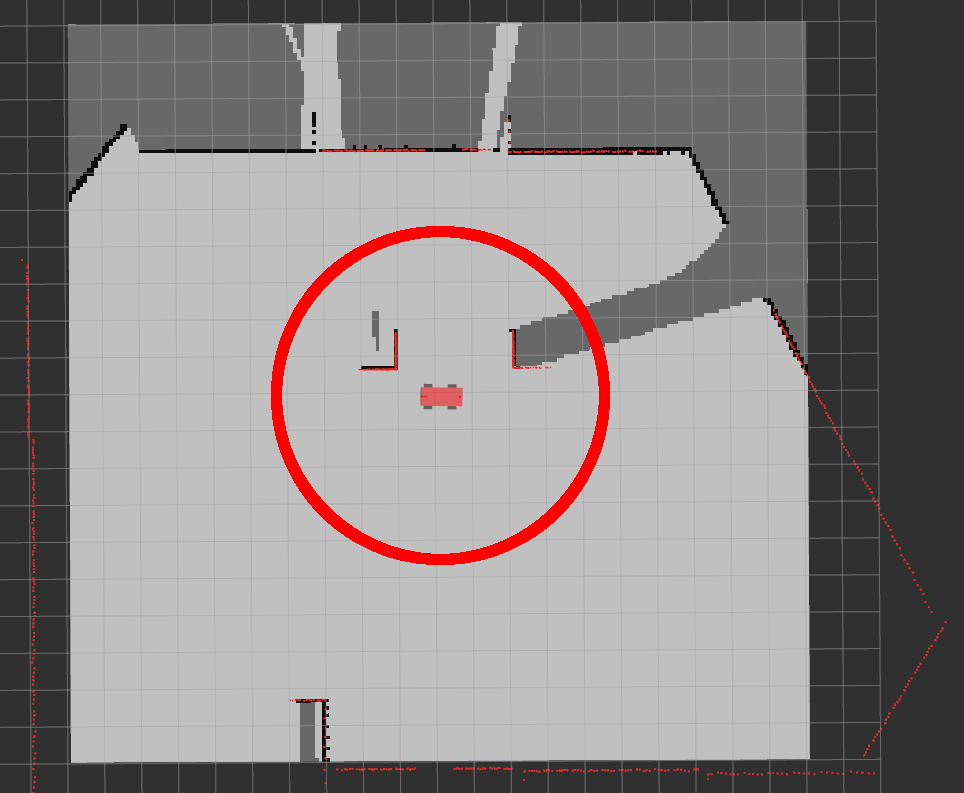
\includegraphics[height=110mm]{figures/raw/rviz_2_near_static_objects_filter.png}
    \caption{Static filtering}
    \label{rviz_2_near_static_objects_filter}
\end{figure}

Figure \ref{rviz_2_near_static_objects_filter} shows that the mapped environment of the car is a much larger territory than what the motion planning algorithm needs to check for collisions. The circle marks the area that is kept after the filtering. In this example, this area contains the two square-shaped obstacles, all the other points in the static map are thrown. The size of the area worth keeping always depends on the actual application and the car's dynamic characteristics. But as a general rule of thumb:

\begin{equation}\label{eq:static_area}
R = \frac{v_{max}^2}{a_{max}}
\end{equation}

\begin{center}
    \begin{tabular}{ | c | c | }
        \hline
        $v_{max}$    & The maximum speed             \\
        \hline
        $a_{max}$    & The maximum deceleration      \\
        \hline
        $R$          & The radius of the kept area   \\
        \hline
    \end{tabular}
\end{center}

is a good guess. The maximum speed and deceleration and settable parameters (see MAX\_SPEED\_FWD, MAX\_SPEED\_BWD and MAX\_ACCELERATION in Section \ref{chap:motion_planner_input_parameters}). Optimization is possible using the car's speed vector, and filtering out those points that are very far from the current direction.

\subsection{Static collision times}
Collision times need to be changed for all surrounding obstacles in order to be able to build the dynamic velocity obstacle map. Due to the fact that the number of static points is usually high compared to the dynamic points, the collision times are calculated separately, so that the calculation can be optimized for static objects. Collision check needs to be executed for all the actuations within the dynamic window. The algorithm is the following.

First the car's expected movement for the actuation is predicted with a curve. When the wheel angle is very close to 0, this curve can be approximated with a straight line, in these cases the algorithm is simplified. However, now let us consider a scenario when the angle is not 0, and the trajectory will in fact be a curve of finite radius. Figure \ref{static_collision_time_check_objects} shows this scenario.

\begin{figure}[!ht]
    \centering
    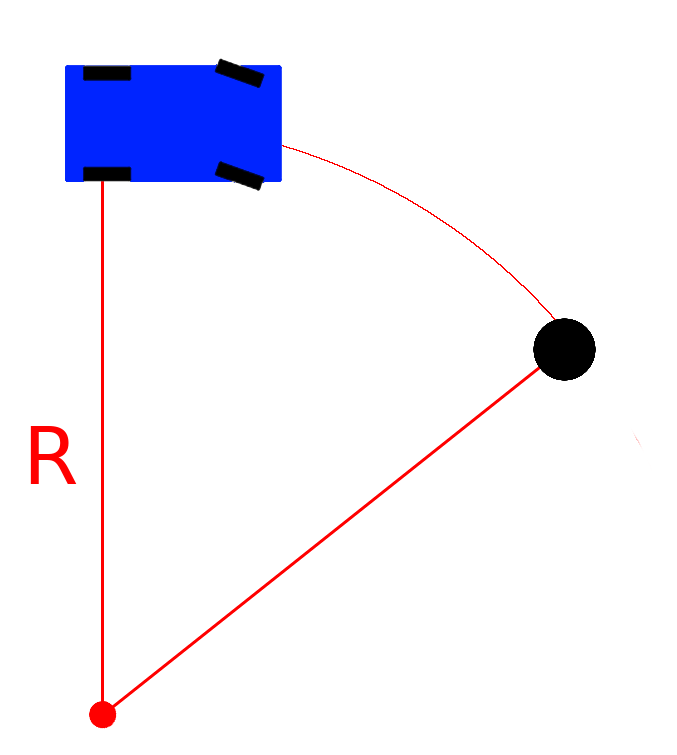
\includegraphics[height=72mm]{figures/raw/static_collision_time_check_objects.png}
    \caption{The car's expected trajectory is a curve}
    \label{static_collision_time_check_objects}
\end{figure}

In order to get the collision time, first the algorithm needs to calculate the collision distance. This calculation is based on linear algebra. But in order to be able apply mathematical laws on the model, the objects need to be converted to simple geometrical forms. This simplification is represented in Figure \ref{static_collision_time_check_object_simplification}.

\begin{figure}[!ht]
    \centering
    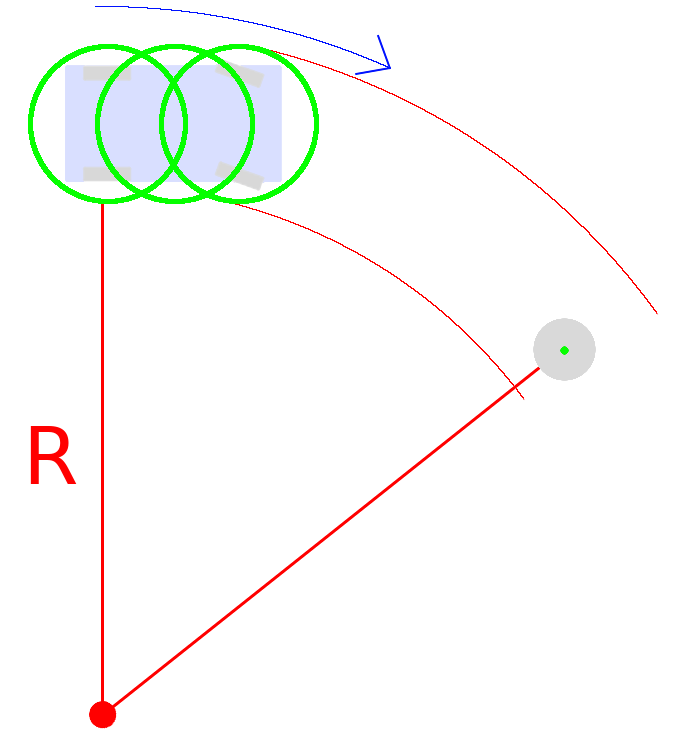
\includegraphics[height=72mm]{figures/raw/static_collision_time_check_object_simplification.png}
    \caption{Simplifying object shapes}
    \label{static_collision_time_check_object_simplification}
\end{figure}

As it is clearly visible on the image, the car is approximated with 3 circles, fixed on the car's axles and its center, and the obstacle is simplified to one circle. In order for easier calculations, the obstacle is not handled as a circle of given radius, but as a point, and its radius is added to the radiuses of the car's circles. We also need to take into consideration, that the static map is always noisy, and we can never expect measurements to be noiseless, either. Therefore, a third value is added to the radiuses of the car's circles, which is the minimal distance that needs to be kept from static objects. Therefore the car circle radius is as follows:

\begin{equation}\label{eq:car_circle_radius}
r = \frac{w_{car}}{2} + r_{obs} + d_{min}
\end{equation}

\begin{center}
    \begin{tabular}{ | c | c | }
        \hline
        $w_{car}$    & The width of the car             \\
        \hline
        $r_{obs}$    & The obstacle radius              \\
        \hline 
        $d_{min}$    & The minimal kept distance        \\
        \hline 
        $r$          & The modified car circle radius   s\\
        \hline
    \end{tabular}
\end{center}

The angular difference between the car and the obstacle (denoted $\gamma$) can be calculated easily (see Figure \ref{static_collision_time_check_angle}).

\begin{figure}[!ht]
    \centering
    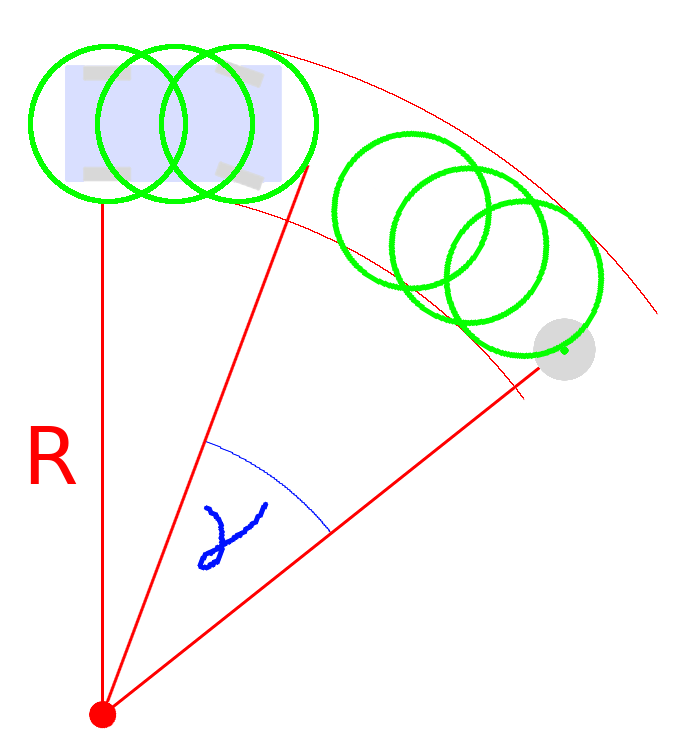
\includegraphics[height=72mm]{figures/raw/static_collision_time_check_angle.png}
    \caption{Angular difference between the car and the obstacle}
    \label{static_collision_time_check_angle}
\end{figure}

After the angle is obtained, the collision distance and time can be easily calculated using the following equations:

\begin{equation}\label{eq:collision_dist}
s_{coll} = R \cdot \gamma
\end{equation}

\begin{equation}\label{eq:collision_time}
t_{coll} = s_{coll} \cdot v_{car}
\end{equation}

\begin{center}
    \begin{tabular}{ | c | c | }
        \hline
        $R$         & The radius of the trajectory curve    \\
        \hline
        $\gamma$    & The angular difference                \\
        \hline
        $s_{coll}$  & The distance until collision          \\
        \hline
        $v_{car}$   & The car speed                         \\
        \hline 
        $t_{coll}$  & The time until collision              \\
        \hline
    \end{tabular}
\end{center}

Using the method described above, the collision times for the static obstacles in the map can be calculated. Doing this for all possible actuations will provide a static velocity obstacle map, which later can be used to grade actuations.

\section{Dynamic velocity obstacle map}
\label{chap:dynamic_velocity_obstacle_map}
Dynamic obstacles are also obtained from the mapping node, on topic \textit{dynamic\_objects} (see \ref{chap:publishing_dynamic_obstacles}).
Handling dynamic obstacles is more difficult than handling static points, the algorithm, however, evaluating the moving objects is more straight-forward than the static method using. The reason for the dynamic algorithm being easier to comprehend is that it uses an iterative approach. (Geometrical equations with multiple objects moving in non-straight paths are not trivial.)

\subsection{Filtering dynamic objects}
This first step when evaluating dynamic objects in the map is similar to static case - removing the too far obstacles. Trajectory modelling and collision check may be  resource and time heavy, so handling as few dynamic objects as possible is crucial. The size of the area worth keeping depends on the actual application and the dynamic characteristics of the car and the other moving objects. But as a general rule of thumb:

\begin{equation}\label{eq:extended_car_radius}
R = 2 \cdot \frac{v_{max}^2}{a_{max}}
\end{equation}

\begin{center}
    \begin{tabular}{ | c | c | }
        \hline
        $v_{max}$    & The maximum speed             \\
        \hline
        $a_{max}$    & The maximum deceleration      \\
        \hline
        $R$          & The radius of the kept area   \\
        \hline
    \end{tabular}
\end{center}

is a good guess (note that the radius is twice as large as in the static case). Some optimizations using the car's speed vector can be made in this case, too, but keeping in mind that dynamic objects can approach from behind as well is important.

\subsection{Trajectory calculation}
\label{trajectory_calculation}
Now that the irrelevant dynamic objects have been filtered out, the next step is to calculate the kept obstacles' trajectories. Trajectory calculation is done using an iterative method - for each obstacle, with a given time step (see COLLISION\_CHECK\_TIME\_STEP in Section \ref{chap:motion_planner_input_parameters}) the algorithm start iterating, updates the obstacle's position and orientation in each step and saves into an array of configurations - this array will become the trajectory itself. \textit{But how many steps should be saved?} may be an interesting question, to which the answer is also: it depends. It depends on how the application logic uses these trajectories. For my application, empirical testing showed that the needed collision time check interval is around 3 times the car's actual brake time, for which the needed number of steps is:

\begin{equation}\label{eq:collision_check_time_max}
T_{check,max} = 3 \cdot \frac{v_{max}}{a_{max}}
\end{equation}

\begin{equation}\label{eq:collision_check_steps_max}
N_{max} = \frac{T_{check,max}}{T_{step}}
\end{equation}

\begin{center}
    \begin{tabular}{ | c | c | }
        \hline
        $v_{max}$       & The maximum speed                     \\
        \hline
        $a_{max}$       & The maximum deceleration              \\
        \hline
        $T_{check,max}$ & The collision time check interval     \\
        \hline
        $T_{step}$      & The trajectory simulation time step   \\
        \hline
        $N_{max}$       & The maximum number of needed steps    \\
        \hline
    \end{tabular}
\end{center}

After the trajectories for all moving obstacles have been calculated, the algorithm can move forward, and check for collisions with these objects.

\subsection{Dynamic collision times}
Calculating the collision times with the dynamic obstacles is not based on geometrical considerations, like in the static case, but is executed in an iterative way. For all possible actuations (actuations that are present in the dynamic window), a trajectory is calculated - the same way that it has already been calculated for the other dynamic objects in the map. Using this trajectory and the pre-calculated other trajectories the algorithm iterates through time, updates the objects' configurations in each step according to their trajectories, and checks collisions. The iteration's time step is the configurable value that has been used before (see COLLISION\_CHECK\_TIME\_STEP in Section \ref{chap:motion_planner_input_parameters}). The simulation time (until the iterations proceed) is:

\begin{equation}\label{eq:collision_check_time}
T_{check} = 3 \cdot \frac{v}{a_{max}}
\end{equation}

\begin{equation}\label{eq:collision_check_steps}
N = \frac{T_{check}}{T_{step}}
\end{equation}

\begin{center}
    \begin{tabular}{ | c | c | }
        \hline
        $v$             & The speed of the current actuation        \\
        \hline
        $a_{max}$       & The maximum deceleration                  \\
        \hline
        $T_{check,max}$ & The collision time check interval         \\
        \hline
        $T_{step}$      & The collision check simulation time step  \\
        \hline
        $N$             & The number of needed steps                \\
        \hline
    \end{tabular}
\end{center}

Given that:

\[ v <= v_{max} \]

\begin{center}
    \begin{tabular}{ | c | c | }
        \hline
        $v_{max}$    & The maximum speed        \\
        \hline
    \end{tabular}
\end{center}

the following statement is always true:

\begin{equation}\label{eq:collision_time_check_smaller_than_max}
N <= \frac{3 \cdot \frac{v_{max}}{a_{max}}}{T_{step}} = N_{max}
\end{equation}

which was the number trajectory simulation time steps for the surrounding obstacles (see \ref{trajectory_calculation}). Therefore, it is provided that all objects in the environment have a pre-calculated trajectory for the whole collision check simulation interval.

\begin{minipage}{\textwidth}
\section{Velocity obstacle map evaluation}
\label{chap:velocity_obstacle_map_evaluation}
Let me summarize briefly what the algorithm has done so far.

In each iterations, the algorithm:
\begin{enumerate}
  \item found a new destination point and updated the target actuation
  \item updated the dynamic window of actuations
  \item received a static map and an array of dynamic obstacles from the mapping node
  \item filtered both in order to keep only the objects relevant for local motion planning
  \item calculated trajectories for all dynamic obstacles
  \item checked all available actuations for collisions with any of the static or dynamic objects
  \item built a velocity obstacle map using these collision times
\end{enumerate}
\end{minipage}

Now the next (and final) step is to evaluate the velocity obstacle map, and find the best actuation. But defining what 'the best' actuation is is not trivial.
Let's look at the scenario represented in Figure \ref{what_is_the_best_actuation}.

\begin{figure}[!ht]
    \centering
    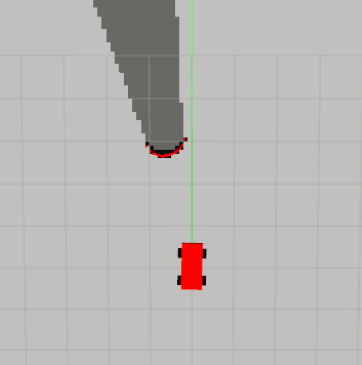
\includegraphics[height=72mm]{figures/raw/rviz_straight_traj_static_object.png}
    \caption{What is 'the best' actuation?}
    \label{what_is_the_best_actuation}
\end{figure}

The target trajectory is a straight line (marked with the green line in the rviz visualization, published by the motion planning node on topic \textit{global\_trajectory}). But there is an obstacle in the way. Without the obstacle being in the picture, one could state without hesitation, the the target actuation is always the one that keeps the car on the line. But once the object is there, this is no longer the case. Defining the best actuation to be the one that keeps car in direction would lead to collision, obviously, the car needs to steer to the right to avoid that. But this raises even more questions. \textit{Should the car steer to the right long before the object? Is it enough to turn the wheels in the last moment? Are we sure we are able to steer away from collision, isn't an emergency brake a better solution?} I answered these questions and solved the problem of finding the best actuation with the introduction of fitness factors.

\subsection{Fitness factors}
A fitness factor is a number in the [0.0 1.0] interval describing how good (how fit) the given actuation is according to an expectation or requirement. I introduced three fitness factors in the algorithm.

\begin{minipage}{\textwidth}
\textbf{Speed factor}

Describes how near the actuation's speed is to the target speed.

\textbf{1.0}: The actuation's speed is exactly the same as the target speed.

\textbf{0.5}: The actuation's speed is halfway between the target speed and the worst possible candidate.

\textbf{0.0}: The actuation's speed is the maximum permitted speed to the opposite direction (worst possible candidate).
\end{minipage}

\begin{minipage}{\textwidth}
\textbf{Direction factor}

Describes how near the actuation's wheel angle is to the target wheel angle.

\textbf{1.0}: The actuation's wheel angle is exactly the same as the target wheel angle.

\textbf{0.5}: The actuation's wheel angle is halfway between the target wheel angle and the worst possible candidate.

\textbf{0.0}: The actuation's wheel angle is the maximum permitted wheel angle to the opposite direction (worst possible candidate).
\end{minipage}

\begin{minipage}{\textwidth}
\textbf{Safety factor}

Describes how safe the actuation is, meaning how improbable a collision is.

\textbf{1.0}: Using the actuation, a collision within time interval will not happen.

\textbf{0.5}: The actuation leads to a collision, but the obstacle is farther than the car's brake distance. Therefore, the collision is avoidable and not critical.

\textbf{0.0}: The actuation leads to an unavoidable collision.
\end{minipage}

Let me explain these factors with two simple examples, regarding the same scenario (shown above in figure Figure \ref{what_is_the_best_actuation}).
The following images show two possible actuations in a situation (both are within the dynamic window). And based on their speed and wheel angles, the car's current configuration and the obstacle's position, the fitness factors can be calculated for both actuations.

\begin{figure}[!ht]
    \centering
    \subfloat[Straight actuation]
    {
        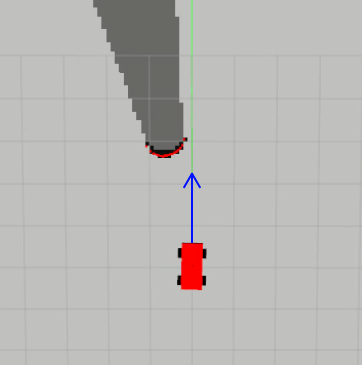
\includegraphics[height=60mm]{figures/raw/rviz_straight_traj_static_object_straight_actuation.png}
        \label{straight_actuation}
    }
    \subfloat[Curved actuation]
    {
        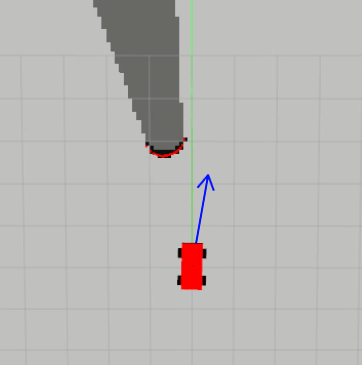
\includegraphics[height=60mm]{figures/raw/rviz_straight_traj_static_object_curved_actuation.png}
        \label{curved_actuation}
    }
    \caption{Possible actuations}
    \label{possible_actuations}
\end{figure}

Figure \ref{possible_actuations} shows the two example actuations. As a precondition, the target speed and wheel angle must be defined. The target speed is always defined by the maximum allowed speed (see MAX\_SPEED\_FWD and MAX\_SPEED\_BWD in Section \ref{chap:motion_planner_input_parameters}) and the target wheel angle. For this is only an example, let me assume that the car is in perfect orientation and arbitrarily set the target speed to MAX\_SPEED\_FWD, and the target wheel angle to zero. Let us assume that we have already calculated the collision times for each possible actuation.

\begin{minipage}{\textwidth}
During factor calculations, the following acronyms are used:

\begin{center}
    \begin{tabular}{ | c | c | }
        \hline
        $MAX\_SPEED\_FWD$    & The maximum permitted forward speed               \\
        \hline
        $MAX\_SPEED\_BWD$    & The maximum permitted backward speed              \\
        \hline
        $MAX\_ACCELERATION$  & The maximum permitted acceleration                \\
        \hline
        $MAX\_WHEEL\_ANGLE$  & The maximum permitted wheel angle                 \\
        \hline
        $T_{check}$          & The collision time check interval                 \\
        \hline
        $v_{target}$         & The target speed                                  \\
        \hline
        $\alpha_{target}$    & The target wheel angle                            \\
        \hline
        $v_{i}$              & The speed of actuation \textit{i}                 \\
        \hline
        $\alpha_{i}$         & The wheel angle of actuation \textit{i}           \\
        \hline
        $t_{coll,i}$         & The collision time using actuation \textit{i}     \\
        \hline
        $F_{speed,i}$        & The speed factor for actuation \textit{i}         \\
        \hline
        $F_{dir,i}$          & The direction factor for actuation \textit{i}     \\
        \hline
        $F_{safety,i}$       & The safety factor for actuation \textit{i}        \\
        \hline
    \end{tabular}
\end{center}
\end{minipage}

\begin{minipage}{\textwidth}
\[ MAX\_SPEED\_FWD = 1.5 \frac{m}{s} \]
\[ MAX\_SPEED\_BWD = -1.5 \frac{m}{s} \]
\[ MAX\_ACCELERATION = 1.5 \frac{m}{s^2} \]
\[ MAX\_WHEEL\_ANGLE = 20° \]
\[ T_{check} = 3 \cdot \frac{MAX\_SPEED\_FWD}{MAX\_ACCELERATION} = 3 s \]
\[ v_{target} = MAX\_SPEED\_FWD \]
\[ \alpha_{target} = 0° \]
\end{minipage}

\begin{minipage}{\textwidth}
Note that for the sake of this example I came up with values that are easy to calculate with. In the real algorithm, for example, $T_{check}$ is calculated from 

Factors for actuation \textit{i} are calculated using the following equations:

\begin{equation}\label{eq:speed_factor}
F_{speed,i} = 1 - \frac{abs(v_{i} - v_{target})}{MAX\_SPEED\_FWD - MAX\_SPEED\_BWD}
\end{equation}

\begin{equation}\label{eq:direction_factor}
F_{dir,i} = 1 - \frac{abs(\alpha_{i} - \alpha_{target})}{2 \cdot MAX\_WHEEL\_ANGLE}
\end{equation}

\begin{equation}\label{eq:safety_factor}
F_{safety,i} = \frac{t_{coll,i}}{T_{check}}
\end{equation}

\end{minipage}

\begin{minipage}{\textwidth}

The factor calculations for the two examples are the following:

\textbf{Straight actuation} (Figure \ref{straight_actuation})

\[ v_{1} = 1.5 \frac{m}{s} \]
\[ \alpha_{1} = 0° \]
\[ t_{coll,1} = 1.5 s \]
\end{minipage}

\begin{minipage}{\textwidth}
The fitness factors are the following (calculated by the Equations \ref{eq:speed_factor}, \ref{eq:direction_factor} and \ref{eq:safety_factor}):

\[ F_{speed,1} = 1.00 \]
\[ F_{dir,1} = 1.00 \]
\[ F_{safety,1} = 0.50 \]
\end{minipage}

As it is clearly visible on the picture, and also from the results, the speed and direction factors are perfect, but the safety factor is low, because the leads to a collision in the near future. Now let us examine the other actuation.

\begin{minipage}{\textwidth}
\textbf{Curved actuation} (Figure \ref{curved_actuation})

\[ v_{2} = 1.5 \frac{m}{s} \]
\[ \alpha_{2} = -10° \]
\[ t_{coll,2} = 4.5 s \]
\end{minipage}

Note that the collision time of the actuation is always in the [0 {$T_{check}$] interval. The result of the collision time check method is T\textsubscript{check} when the actuation does not cause a collision. The fitness factors are the following (calculated by the equations listed above):

\[ F_{speed,2} = 1.00 \]
\[ F_{dir,2} = 0.75 \]
\[ F_{safety,2} = 1.00 \]

Now that the speed, direction and safety factors have been calculated for all possible actuations, the only sub-task left is to find the best actuation.

\begin{minipage}{\textwidth}
\subsection{The best actuation}

The best possible actuation is always the one with the highest fitness factors. The factors of an actuation are summarized to one number (which will then become \textit{the} fitness of the actuation) the following way:

\begin{equation}\label{eq:fitness_factor}
F_{i} = \frac{F_{speed,i} \cdot w_{speed} + F_{dir,i} \cdot w_{dir} + F_{safety,i} \cdot w_{safety}}{w_{speed} + w_{dir} + w_{safety}}
\end{equation}

\end{minipage}

\begin{center}
    \begin{tabular}{ | c | c | }
        \hline
        $F_{i}$         & The fitness of actuation \textit{i}                                                                                     \\
        \hline
        $F_{speed,i}$   & The speed factor for actuation \textit{i}                                                                               \\
        \hline
        $F_{dir,i}$     & The direction factor for actuation \textit{i}                                                                           \\
        \hline
        $F_{safety,i}$  & The safety factor for actuation \textit{i}                                                                              \\
        \hline
        $w_{speed}$     & The weight of the speed factor (see W\_SPEED\_FACTOR in Section \ref{chap:motion_planner_input_parameters})             \\
        \hline
        $w_{dir}$       & The weight of the direction factor (see W\_DIRECTION\_FACTOR in Section \ref{chap:motion_planner_input_parameters})     \\
        \hline
        $w_{safety}$    & The weight of the safety factor (see W\_SAFETY\_FACTOR in Section \ref{chap:motion_planner_input_parameters})           \\
        \hline
    \end{tabular}
\end{center}

\begin{minipage}{\textwidth}
In the implementation, the weights are set as follows. (Further tuning is possible and advised for more production-ready implementations.)

\[ W\_SPEED\_FACTOR = 2.00 \]
\[ W\_DIRECTION\_FACTOR = 1.00 \]
\[ W\_SAFETY\_FACTOR = 4.00 \]
\end{minipage}

As an example, let us continue the previous example with the straight and the curved actuations.

\begin{minipage}{\textwidth}
\textbf{Straight actuation} (Figure \ref{straight_actuation})

\[ F_{speed,1} = 1.00 \]
\[ F_{dir,1} = 1.00 \]
\[ F_{safety,1} = 0.50 \]

An the final fitness is:

\[ F_{1} = \frac{1.00 \cdot 2.00 + 1.00 \cdot 1.00 + 0.50 \cdot 4.00}{2.00 + 1.00 + 4.00} = 0.71 \]
\end{minipage}

\begin{minipage}{\textwidth}
\textbf{Curved actuation} (Figure \ref{curved_actuation})

\[ F_{speed,2} = 1.00 \]
\[ F_{dir,2} = 0.75 \]
\[ F_{safety,2} = 1.00 \]

An the final fitness is:

\[ F_{2} = \frac{1.00 \cdot 2.00 + 0.75 \cdot 1.00 + 1.00 \cdot 4.00}{2.00 + 1.00 + 4.00} = 0.96 \]
\end{minipage}

The results show that out these two actuations, the second one (the curve) would have been selected by the algorithm. This is mainly because safety has a much higher weight than direction when summarizing factors. Obviously, this has not been a complete actuation search because the example consisted of only two actuations, while the the dynamic window can consist of tens or even hundreds of possible alternatives. As I mentioned earlier, the width and the height of the dynamic window depends on the car's and the environments characteristics, while its resolution can be set in the parameters (see DYNAMIC\_WINDOW\_ANGLE\_RESOLUTION and DYNAMIC\_WINDOW\_SPEED\_RESOLUTION in Section \ref{chap:motion_planner_input_parameters}).

\subsection{Publishing Ackermann driving control}
The hard part of the node's work is done, the best possible actuation has been found. The very last task is to publish this desired speed and wheel angle pair to the other ROS nodes that control the car.

This publication happens on topic \textit{/vrcar/manual\_control}, using \href{http://docs.ros.org/jade/api/ackermann_msgs/html/msg/AckermannDrive.html}{\textit{ackermann\_msgs/AckermannDrive}} messages.

The actuator nodes will use these messages to propagate the requested values to the DC motor and the steering servo, and thus, the control pipe has reached its end.